\section{Introduction}
\label{sec:introduction}

Large Language Models (LLMs) have the potential to help scientists with retrieving, synthesizing, and summarizing the scientific literature \cite{skarlinski_language_2024}. 
However, issues such as hallucinations \cite{pmlr-v202-shi23a} \cite{xu_hallucination_2025}, and underdeveloped retrieval and reasoning benchmarks, hamper the direct use of LLMs in scientific research . \\

The field is rapidly developing, with new models such as Google's Gemini 2.5 and OpenAI's o3 being able to 'reason', and excel at coding, maths, and language benchmarks. 
This also highlights the developments of new cutting-edge benchmarks for scientific performance in areas such as scientific discovery \cite{shojaee_llm-srbench_2025}, analysis \cite{cai_sciassess_2024}, programming \cite{openai_competitive_2025}, \cite{quan_codeelo_2025}, and mathematics \cite{liu_mathbench_2024}. \\

Alongside the development of the fundamental models themselves, techniques such as Retrieval Augmented Generation (RAG) and the use of Multi-Agent Systems (MAS) allowed better use of LLMs in scientific research. \\

\subsection{Retrieval Augmented Generation}
Retrieval Augmented Generation (RAG) is a sophisticated technique designed to enhance the capabilities of Large Language Models (LLMs) by grounding their responses in external knowledge sources. This process mitigates common LLM issues like hallucinations and outdated information by dynamically providing relevant, fact-based context. The RAG process can be broken down into several key stages \cite{gupta_comprehensive_2024} \cite{lewis_retrieval-augmented_2021}.

\begin{enumerate}
    \item \textbf{Indexing}: A corpus of documents (e.g., scientific papers, reports, web pages) is processed into a searchable format. This involves loading the documents, splitting them into smaller, manageable chunks of text, and converting these chunks into numerical representations called vector embeddings using an embedding model. These embeddings are then stored in a specialized vector database, which allows for efficient similarity searching.
    \item \textbf{Retrieval}: When a user submits a query, it is also converted into a vector embedding using the same model. The vector database is then searched to find the document chunks with embeddings that are most similar to the query embedding. This similarity search efficiently identifies the most relevant information in the knowledge base.
    \item \textbf{Augmentation and Generation}: The retrieved document chunks are then combined with the original user prompt and fed as context to an LLM. The model uses this augmented prompt to generate a response that is synthesized directly from the provided information, ensuring the answer is relevant, accurate, and grounded in the source material.
\end{enumerate}

This architecture is powerful because it separates the knowledge base from the generative model, allowing the knowledge to be updated without needing to retrain the LLM.

\begin{figure}[H]
    \centering
    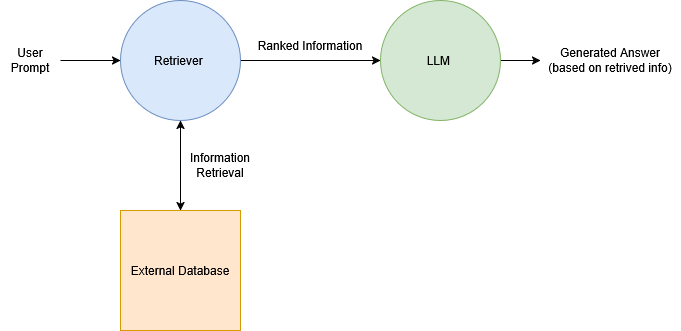
\includegraphics[width=\textwidth]{figures/basic_rag.png}
    \caption{A basic RAG pipeline. The user query is converted into a vector embedding, which is then used to search the vector database for the most relevant document chunks. These chunks are then combined with the original user prompt and fed as context to an LLM. The model uses this augmented prompt to generate a response that is synthesized directly from the provided information.}
    \label{fig:basic_rag}
\end{figure}

\subsection{Multi-Agent Systems}
Multi-Agent Systems (MAS) represent a shift from using a single LLM to orchestrating multiple, specialized LLM-powered agents that collaborate to solve complex problems. This approach is analogous to a team of human experts, where each member has a specific role and set of tools. Instead of being "trained" in the traditional sense, these agents are \textit{instructed} through carefully crafted prompts that define their roles, goals, and constraints. Their power comes from a well-defined system of interaction and tool use \cite{han_llm_2025}.\\

The development of a MAS typically involves three key components:
\begin{enumerate}
    \item \textbf{Role Specialization}: Each agent is given a specific persona or role (e.g., "Planner," "Code Critic," "Financial Analyst") through its system prompt. This focuses the agent's behavior on a specific part of the problem.
    \item \textbf{Tool Use}: Agents are equipped with specific tools, such as web search APIs, code interpreters, or private knowledge bases, allowing them to interact with the outside world and perform actions beyond text generation.
    \item \textbf{Orchestration/Planning}: A framework is used to manage how the agents collaborate. This can be a hierarchical structure where a "manager" agent delegates tasks, a sequential process where tasks are passed down a pipeline, or a conversational "group chat" where agents can interact more dynamically.
\end{enumerate}

Several powerful frameworks have emerged to facilitate the creation of these systems. \textbf{Microsoft's AutoGen} \cite{wu_autogen_2023} excels at creating flexible, conversation-based agents that can dynamically interact. \textbf{LangGraph}, \cite{wang_agent_2024} an extension of the popular LangChain library, provides more explicit control by allowing developers to define workflows as stateful graphs, which is ideal for complex and cyclical processes. \textbf{CrewAI} offers a more intuitive, high-level abstraction, focusing on creating a "crew" of agents with predefined roles to tackle tasks in a structured, sequential manner. These tools mark a major leap forward toward automated scientific discovery and complex problem-solving. \\

\subsection{PaperQA2}
To make scientific discoveries, one must be able to synthesise scientific knowledge.
Skarlinski et. al. believe this can be broken down into three vital tasks: scientific question answering, summarising, and detecting contradictions in the literature.
In their paper, it is shown that their developed tool, PaperQA2, outperforms the human benchmark in all three areas \cite{skarlinski_language_2024}. 
The focus of this report is to understand and reproduce the question-answering result. \\

\subsubsection{PaperQA2 Architecture}
PaperQA2 operates as an agentic Retrieval-Augmented Generation (RAG) system built upon the \texttt{paperqa} Python package. Its architecture enables a flexible workflow where an agent can operate on a pre-indexed local corpus or dynamically search for and ingest new documents at query time. The typical agentic query process involves the following stages:\\

\textbf{1. Paper Search and Dynamic Ingestion:}
The agent's workflow begins by invoking a search tool, such as one that interfaces with the \texttt{Semantic Scholar} API. The agent first uses an LLM to distill the user's query into a set of precise keywords. These keywords are used to query the external academic database, which returns a list of candidate papers. The agent then retrieves the relevant documents (e.g., as PDFs) and parses them to extract their content. While the framework includes a built-in \texttt{PyMuPDF} parser for text extraction, it can also be integrated with more advanced external tools like \texttt{Grobid}, which can parse the full document structure (e.g., title, sections, references). The extracted text is then segmented into configurable, overlapping chunks. These chunks are immediately converted into vector embeddings using a configurable model and indexed in both a keyword store (\texttt{tantivy}) and a vector store (\texttt{Numpy} or \texttt{Qdrant}). This on-the-fly ingestion process makes the newly found papers available for the subsequent stages of the current query. \\

\textbf{2. Evidence Gathering and Re-ranking:}
With a set of newly ingested chunks available, the system proceeds to a multi-step evidence-gathering phase to refine the context. This involves:
\begin{itemize}
    \item \textbf{Vector and Hybrid Search:} A vector cosine similarity search is performed on the candidate chunks. The framework supports \textbf{hybrid search}, a technique that combines two different kinds of vectors for ranking. It uses dense vector embeddings, which capture the semantic or conceptual meaning of the text, along with sparse keyword-based vectors (e.g., TF-IDF or SPLADE-style models?), which excel at exact term matching. By merging scores from both, hybrid search retrieves chunks that are both thematically related and contain precise keywords from the query. 
    \item \textbf{Result Diversification:} To prevent the retrieval of highly redundant information from a single source, the system can apply \textbf{Maximal Marginal Relevance (MMR)}. Instead of just optimizing for similarity to the query, MMR iteratively selects chunks by balancing their relevance with their novelty compared to chunks already selected. This ensures the resulting evidence set is both on-topic and informationally diverse.
    \item \textbf{LLM-based Re-ranking and Contextual Summarization (RCS):} This is arguably the most critical and computationally intensive step, invoked by a \texttt{GatherEvidence} tool. The top \textit{k} chunks from the previous steps (a number configurable via \texttt{answer.evidence\_k}) are not used directly. Instead, each individual chunk is passed to an LLM with a specific prompt instructing it to summarize the chunk's content strictly in relation to the user's original query and to assign a relevance score. This use of an LLM as a "re-ranker" is highly effective at filtering out passages that may be semantically similar but not actually useful for answering the question, while simultaneously distilling the most important information.
\end{itemize}

\textbf{3. Answer Generation:}
In the final stage, a \texttt{GenerateAnswer} tool compiles the highest-scoring summaries from the RCS step into a single context. The number of evidence pieces included is configurable via parameters like \texttt{answer.answer\_max\_sources}. This context, along with the original question, is formatted into a final prompt using a customizable template (\texttt{prompt.qa}). This allows for fine-grained control over how the LLM is instructed to synthesize the information. The model then generates a comprehensive answer that is directly grounded in the selected sources. The system formats this answer with inline citations that trace back to the original documents, providing a verifiable response. \\

\textbf{4. Citation Traversal:}
As an optional step, the agent can employ a \textbf{Citation Traversal} tool to expand the scope of its search beyond the initial document corpus. After identifying a highly relevant paper, this tool can be used to analyze its bibliography or query external databases (like Semantic Scholar) to find papers it cites (backward traversal) or papers that cite it (forward traversal). This is a technique for discovering foundational research or, conversely, the latest developments building upon a known paper. These newly discovered documents can then be ingested and indexed as it runs, allowing the agent to dynamically expand its knowledge base to answer a query more comprehensively. \\

\subsubsection{Key Result}
The paper claims that PaperQA's performance beats the human benchmark, specifically for the precision of questions answered, achieving a precision of 85.2\% compared to the human precision of 73.8\%. The benchmark metrics are accuracy and precision. \\

\begin{equation}
    Accuracy = \frac{Correct Questions}{All Questions}
\end{equation}


\begin{equation}
    Precision = \frac{Correct Questions}{Answered Questions}
\end{equation}

The process of evaluating the performance of PaperQA2 was to ask questions, where the answers were found in newly published papers and could not be inferred from either the title, abstract, or conclusion.
The questions would also require some 'reasoning' and the answer could not be a direct quote from the paper.  
The questions were taken from recently published biology papers, post September 2021 (the GPT training cutoff). The assumed reason for this is to prevent the LLM agents from using their 'own knowledge', instead of reading and understanding the papers given to it. \\

Human evaluators were then tasked with answering the same questions. 
However, the human evaluators were not directly given the correct paper (or the correct paper within a group of papers, which is essentially how PaperQA performs evaluation). 
Instead, the evaluators were access to the internet and journal collections, but were told to not use generative AI tools such as ChatGPT.\\

The aim of this project is to recreate this result, and confirm whether language agents can outperform human performance in question answering. \\

